After conducting the measurements, profiles showing the drag coefficient as a function of the wind velocity could be created for each set of disks. 




\section{Rotational WT model}

The first measurement conducted using three rotating WT models resulted in a drag coefficient that was relatively independent of wind velocity for four of the measured wind velocities, but with a significant deviation at 5 m/s. To investigate whether this deviation was due to a measurement error, a second measurement was conducted, this time using three new rotating WT models. This second measurement gave more of an expected result at 5 m/s, however showed a deviation at 15 m/s. Thus, a third measurement, once again with three new rotating WT models, was conducted. Finally, a fourth measurement was carried out, this time using the same models as during the third measurement. The resulting drag coefficients can be seen as a function of wind velocity in figure \ref{fig:RotationalCD}.

\begin{figure}[h!]
    \centering
    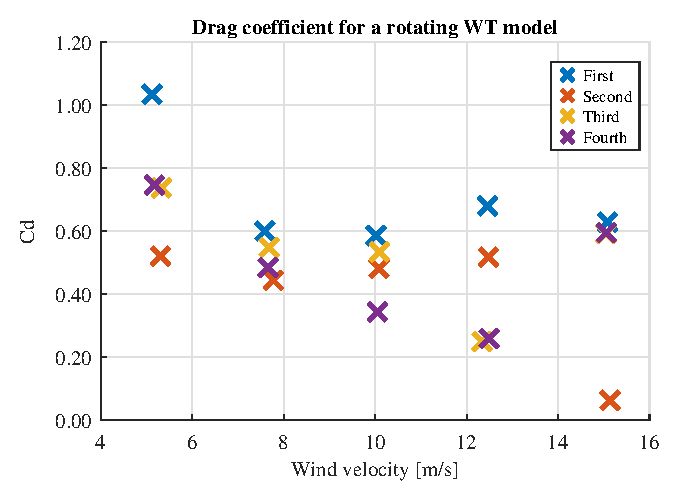
\includegraphics[width=\linewidth]{0_Images/RotationalCD.eps}
    \caption{The drag coefficient for the rotating WT models, obtained through four rounds of measurements.}
    \label{fig:RotationalCD}
\end{figure}

As can be seen, there is some variation between the different measurement point. The values from the third and the fourth measurement are quite similar at 5 m/s, 7.5 m/s and 12 m/s, and at 15 m/s, they completely overlap. This may show that the measurement is repeatable, and that one of the reasons for the varying results is simply that the rotating WT models have small differences, for example related to the friction of the rotating blades and how well they are connected. Be it too tight, there will be added friction. Be it too loose, the blades may start to vibrate. However, even between the third and fourth measurement, there is a noticeable difference at 7.5 m/s, showing that differences between the WT models is not the only cause for the varying results. 

Other possible causes of this variation may be related to noise and fluctuations in the applied wind velocity and in the force plate. 

To investigate the results further, the drag resulting from the different measurements are pictured as a function of wind velocity in figure \ref{fig:RotationalDrag}


\begin{figure}[h!]
    \centering
    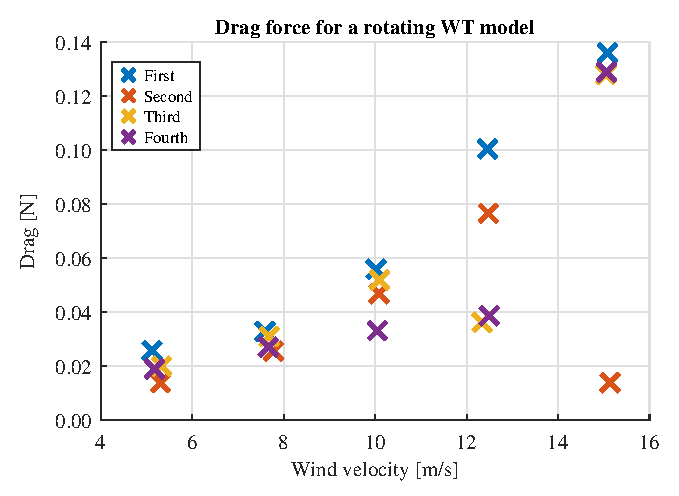
\includegraphics[width=\linewidth]{0_Images/RotationalDrag.eps}
    \caption{The measured drag for the rotating WT models, obtained through four rounds of measurements.}
    \label{fig:RotationalDrag}
\end{figure}

As can be seen, the drag at 12.5 m/s is lower than the drag at 10 m/s for the third measurement, and the drag at 15 m/s is lower than the drag for 12.5 m/s for the second measurement. This is not physical, and thus it is assumed that these two values are errors. The drag measured during the fourth measurement coinsides with the disregarded drag from the third measurement, and is thus also regarded as an outlier. The wind tunnel did, for some unknown reason, seem to produce larger amounts of noise on the signal for velocities between 11 and 13 m/s. The drag at 10 m/s for the fourth measurement is higher than the drag at 7.5 m/s, however the value is lower than for all the measurements which seem to coincide quite well, and thus this value is considered as an outlier. The initial suspicious value, measured at 5 m/s in the first measurement, results in a $C_d$ larger than one, which seems unlikely, and hence this value is also regarded as an outlier. 

The outlier seem to be spread out both in terms of velocity at which they occur and in terms of whether they exceed or fall below the other values. One can argue that if taking a large number of new measurements, they would have a Gaussian distribution about a mean, and that taking the average of the values that seemingly coincide would be representative for this total mean. %Should probably be extended 

Thus, in order to achieve a representative value for the drag coefficient of the rotating WT models, the outliers were removed, and the average of the remaining drag coefficients was taken. This resulted in the drag coefficients seen in figure \ref{fig:RotationalAvg}.

\begin{figure}[h!]
    \centering
    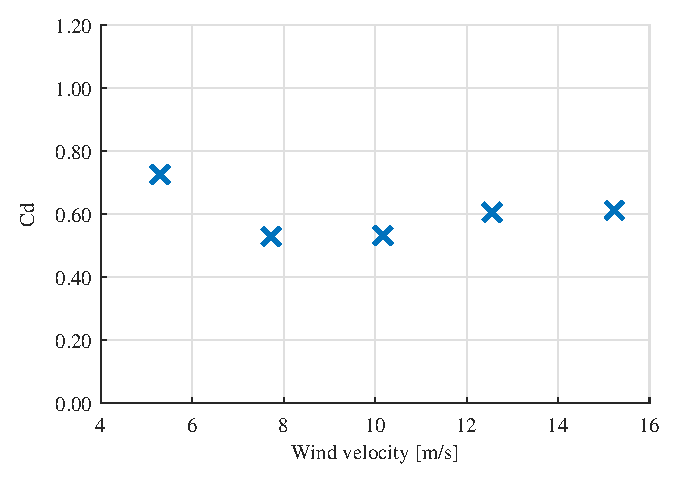
\includegraphics[width=\linewidth]{0_Images/RotationalAverage.eps}
    \caption{The average drag coefficient for the rotational WT models for each wind velocity, based on the four conducted measurements, after removing the assumed wrongful outliers.}
    \label{fig:RotationalAvg}
\end{figure}

Assuming that $C_d$ is Reynolds number independent for such a short span at Reynolds numbers, the average over these measurement points is taken, resulting in an average $C_d$ of 0.585. Based on all the applied values, the standard deviation at hand is... Thus, when creating the ADs, this is the desired drag coefficient. 




\section{Drag on the ADs}
The drag coefficient on the produced ADs has been studied. Initially, the solid disk, used as a reference case, produced the drag seen in figure \ref{Fig:SolidDrag} and the drag coefficient seen in figure \ref{Fig:SolidCD}. Further, the drag and the drag coefficient for the two types of disks with 60\% solidity can be seen in figure \ref{Fig:SixtyDrag} and \ref{Fig:SixtyCD}, respectively. For both, the drag is seen to increase with increasing wind velocity, as one would expect. 



\begin{figure} [h!]
    \centering
    \begin{subfigure}[b]{0.45\linewidth}
        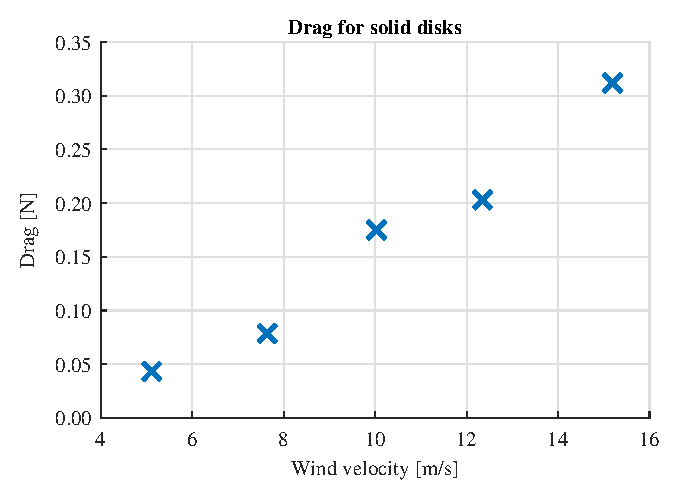
\includegraphics[width=\textwidth]{0_Images/SolidDrag.eps}
        \label{Fig:SolidDrag}
        \caption{The drag.}
    \end{subfigure}
    ~
    \begin{subfigure}[b]{0.45\linewidth}
        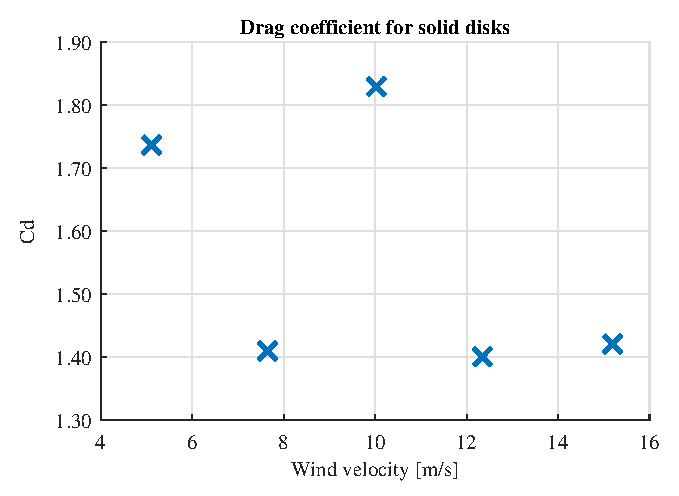
\includegraphics[width=\textwidth]{0_Images/SolidCD.eps}
        \label{Fig:SolidCD}
        \caption{The drag coefficient.}
    \end{subfigure}
    \caption{Using the solid disk.}
    \label{fig:SolidDisk}
\end{figure}

\begin{figure} [h!]
    \centering
    \begin{subfigure}[b]{0.45\linewidth}
        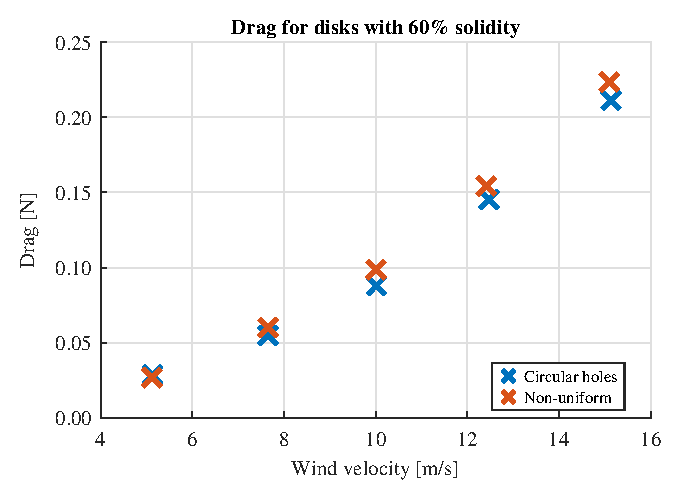
\includegraphics[width=\textwidth]{0_Images/SixtyDrag.eps}
        \label{Fig:SixtyDrag}
        \caption{The drag.}
    \end{subfigure}
    ~
    \begin{subfigure}[b]{0.45\linewidth}
        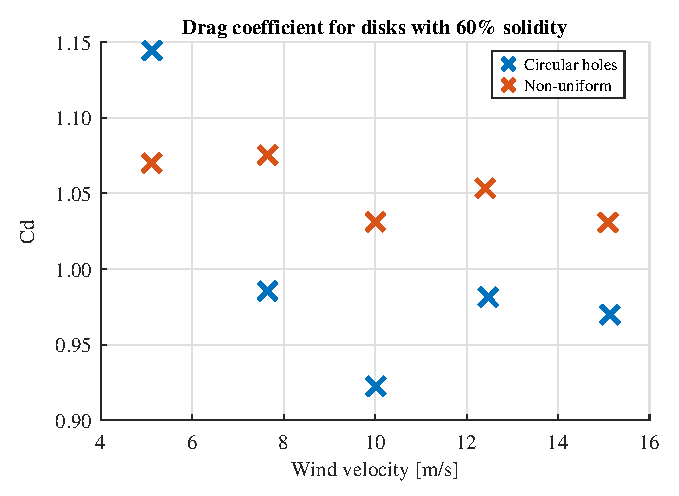
\includegraphics[width=\textwidth]{0_Images/SixtyCD.eps}
        \label{Fig:SixtyCD}
        \caption{The drag coefficient.}
    \end{subfigure}
    \caption{Using the disks with 60\% solidity.}
    \label{fig:SixtyDisk}
\end{figure}


\begin{figure}[h!]
    \centering
    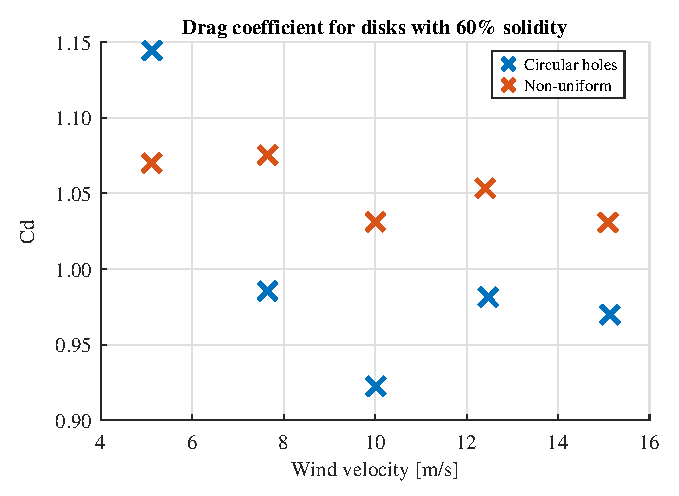
\includegraphics[width=\linewidth]{0_Images/SixtyCD.eps}
    \caption{The drag coefficient for the disks with 60\% solidity.}
    \label{fig:RotationalAvg}
\end{figure}


\begin{figure}[h!]
    \centering
    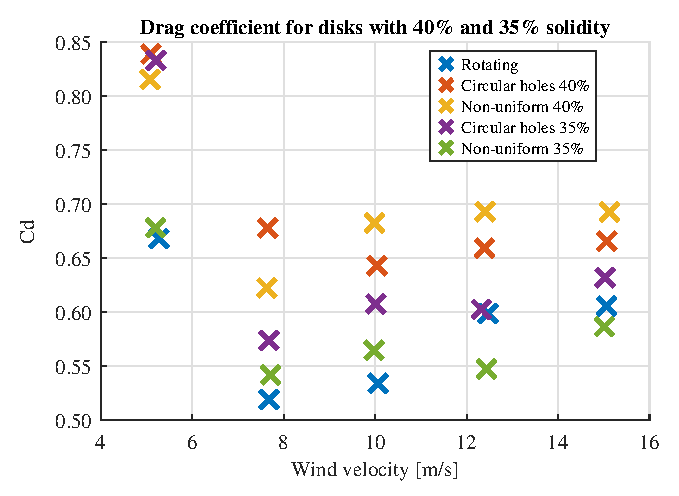
\includegraphics[width=\linewidth]{0_Images/FortyCD.eps}
    \caption{The drag coefficient for the disks with 40\% and 35\% solidity, compared to the average drag coefficient of the rotating disks.}
    \label{fig:RotationalAvg}
\end{figure}


\section{Noise}





%As can readily be seen, the drag coefficient decreases as the solidity of the actuator disks decreases. Vis det 

%This one fits the best. However, the profiles do not look exactly the same. 

%Error, standard deviation 

%why do we get the results that we get? 

%- Cd
%- Drag
%- Adjusting for drift 
%- statistikk arument 
%- usikkerhet


\section{Possible sources of error}
Temperature changes 

